
\documentclass[border=8pt, multi, tikz]{standalone}
\usepackage{import}
\subimport{layers/}{init}
\usetikzlibrary{positioning}
\usetikzlibrary{3d} %for including external image
\usetikzlibrary{calc}

\def\ConvColor{rgb:yellow,5;red,2.5;white,5}
\def\ConvReluColor{rgb:yellow,5;red,5;white,5}
\def\PoolColor{rgb:red,1;black,0.3}
\def\UnpoolColor{rgb:blue,2;green,1;black,0.3}
\def\FcColor{rgb:blue,5;red,2.5;white,5}
\def\FcReluColor{rgb:blue,5;red,5;white,4}
\def\SoftmaxColor{rgb:magenta,5;black,7}

\newcommand{\copymidarrow}{\tikz \draw[-Stealth,line width=0.8mm,draw={rgb:blue,4;red,1;green,1;black,3}] (-0.3,0) -- ++(0.3,0);}

\begin{document}
\begin{tikzpicture}
\tikzstyle{connection}=[ultra thick,every node/.style={sloped,allow upside down},draw=\edgecolor,opacity=0.7]
\tikzstyle{copyconnection}=[ultra thick,every node/.style={sloped,allow upside down},draw={rgb:blue,4;red,1;green,1;black,3},opacity=0.7]

\node[canvas is zy plane at x=0][opacity=1] (temp) at (-1,0,0) {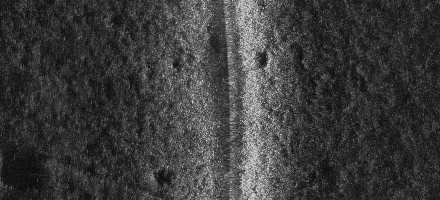
\includegraphics[width=4.4cm,height=2.0cm]{13_0_img.png}};

\pic[shift={(0,0,0)}] at (0,0,0)
    {Box={
        name=Atrous,
        caption= ,
        xlabel={{12, }},
        zlabel=440,
        fill=\ConvReluColor,
        height=10.0,
        width=1,
        depth=22.0
        }
    };

\pic[shift={(1,0,0)}] at (Atrous-east)
    {Box={
        name=db1_0,
        caption= ,
        xlabel={{22, }},
        zlabel=440,
        fill=\ConvColor,
        height=10.0,
        width=1,
        depth=22.0
        }
    };

\pic[shift={(.25,0,0)}] at (db1_0-east)
    {Box={
        name=db1_1,
        caption= ,
        xlabel={{22, }},
        zlabel=440,
        fill=\ConvColor,
        height=10.0,
        width=1,
        depth=22.0
        }
    };

\pic[shift={(.25,0,0)}] at (db1_1-east)
    {Box={
        name=db1_2,
        caption= ,
        xlabel={{22, }},
        zlabel=440,
        fill=\ConvColor,
        height=10.0,
        width=1,
        depth=22.0
        }
    };

\pic[shift={(.25,0,0)}] at (db1_2-east)
    {Box={
        name=db1_3,
        caption= ,
        xlabel={{22, }},
        zlabel=440,
        fill=\ConvColor,
        height=10.0,
        width=1,
        depth=22.0
        }
    };

\pic[shift={(.25,0,0)}] at (db1_3-east)
    {Box={
        name=db1_4,
        caption= ,
        xlabel={{22, }},
        zlabel=440,
        fill=\ConvColor,
        height=10.0,
        width=1,
        depth=22.0
        }
    };

\pic[shift={(.5,0,0)}] at (db1_4-east)
    {Box={
        name=db1_concat,
        caption= ,
        xlabel={{122, }},
        zlabel=440,
        fill=\SoftmaxColor,
        height=10.0,
        width=1,
        depth=22.0
        }
    };

\path (Atrous-southeast) -- (Atrous-northeast) coordinate[pos=1.1400000000000001] (Atrous-top);

\path (db1_0-southwest) -- (db1_0-northwest) coordinate[pos=1.28] (db1_0-top);

\path (db1_1-southwest) -- (db1_1-northwest) coordinate[pos=1.42] (db1_1-top);

\path (db1_2-southwest) -- (db1_2-northwest) coordinate[pos=1.56] (db1_2-top);

\path (db1_3-southwest) -- (db1_3-northwest) coordinate[pos=1.7000000000000002] (db1_3-top);

\path (db1_4-southwest) -- (db1_4-northwest) coordinate[pos=1.84] (db1_4-top);

\path (db1_concat-southwest) -- (db1_concat-northwest) coordinate[pos=1.98] (db1_concat-top);

\draw [red]   (Atrous-northeast) to[out=90, in=180] ($(Atrous-top)!0.5!(db1_0-top)$);
\draw [red]   ($(Atrous-top)!0.5!(db1_0-top)$) to[out=0, in=90 ] (db1_0-northwest);

\draw [red]   (Atrous-northeast) to[out=90, in=180] ($(Atrous-top)!0.5!(db1_1-top)$);
\draw [red]   ($(Atrous-top)!0.5!(db1_1-top)$) to[out=0, in=90 ] (db1_1-northwest);

\draw [red]   (Atrous-northeast) to[out=90, in=180] ($(Atrous-top)!0.5!(db1_2-top)$);
\draw [red]   ($(Atrous-top)!0.5!(db1_2-top)$) to[out=0, in=90 ] (db1_2-northwest);

\draw [red]   (Atrous-northeast) to[out=90, in=180] ($(Atrous-top)!0.5!(db1_3-top)$);
\draw [red]   ($(Atrous-top)!0.5!(db1_3-top)$) to[out=0, in=90 ] (db1_3-northwest);

\draw [red]   (Atrous-northeast) to[out=90, in=180] ($(Atrous-top)!0.5!(db1_4-top)$);
\draw [red]   ($(Atrous-top)!0.5!(db1_4-top)$) to[out=0, in=90 ] (db1_4-northwest);

\draw [red]   (Atrous-northeast) to[out=90, in=180] ($(Atrous-top)!0.5!(db1_concat-top)$);
\draw [red]   ($(Atrous-top)!0.5!(db1_concat-top)$) to[out=0, in=90 ] (db1_concat-northwest);

\path (db1_0-southeast) -- (db1_0-northeast) coordinate[pos=1.1400000000000001] (db1_0-top);

\path (db1_1-southwest) -- (db1_1-northwest) coordinate[pos=1.28] (db1_1-top);

\path (db1_2-southwest) -- (db1_2-northwest) coordinate[pos=1.42] (db1_2-top);

\path (db1_3-southwest) -- (db1_3-northwest) coordinate[pos=1.56] (db1_3-top);

\path (db1_4-southwest) -- (db1_4-northwest) coordinate[pos=1.7000000000000002] (db1_4-top);

\path (db1_concat-southwest) -- (db1_concat-northwest) coordinate[pos=1.84] (db1_concat-top);

\draw [red]   (db1_0-northeast) to[out=90, in=180] ($(db1_0-top)!0.5!(db1_1-top)$);
\draw [red]   ($(db1_0-top)!0.5!(db1_1-top)$) to[out=0, in=90 ] (db1_1-northwest);

\draw [red]   (db1_0-northeast) to[out=90, in=180] ($(db1_0-top)!0.5!(db1_2-top)$);
\draw [red]   ($(db1_0-top)!0.5!(db1_2-top)$) to[out=0, in=90 ] (db1_2-northwest);

\draw [red]   (db1_0-northeast) to[out=90, in=180] ($(db1_0-top)!0.5!(db1_3-top)$);
\draw [red]   ($(db1_0-top)!0.5!(db1_3-top)$) to[out=0, in=90 ] (db1_3-northwest);

\draw [red]   (db1_0-northeast) to[out=90, in=180] ($(db1_0-top)!0.5!(db1_4-top)$);
\draw [red]   ($(db1_0-top)!0.5!(db1_4-top)$) to[out=0, in=90 ] (db1_4-northwest);

\draw [red]   (db1_0-northeast) to[out=90, in=180] ($(db1_0-top)!0.5!(db1_concat-top)$);
\draw [red]   ($(db1_0-top)!0.5!(db1_concat-top)$) to[out=0, in=90 ] (db1_concat-northwest);

\path (db1_1-southeast) -- (db1_1-northeast) coordinate[pos=1.1400000000000001] (db1_1-top);

\path (db1_2-southwest) -- (db1_2-northwest) coordinate[pos=1.28] (db1_2-top);

\path (db1_3-southwest) -- (db1_3-northwest) coordinate[pos=1.42] (db1_3-top);

\path (db1_4-southwest) -- (db1_4-northwest) coordinate[pos=1.56] (db1_4-top);

\path (db1_concat-southwest) -- (db1_concat-northwest) coordinate[pos=1.7000000000000002] (db1_concat-top);

\draw [red]   (db1_1-northeast) to[out=90, in=180] ($(db1_1-top)!0.5!(db1_2-top)$);
\draw [red]   ($(db1_1-top)!0.5!(db1_2-top)$) to[out=0, in=90 ] (db1_2-northwest);

\draw [red]   (db1_1-northeast) to[out=90, in=180] ($(db1_1-top)!0.5!(db1_3-top)$);
\draw [red]   ($(db1_1-top)!0.5!(db1_3-top)$) to[out=0, in=90 ] (db1_3-northwest);

\draw [red]   (db1_1-northeast) to[out=90, in=180] ($(db1_1-top)!0.5!(db1_4-top)$);
\draw [red]   ($(db1_1-top)!0.5!(db1_4-top)$) to[out=0, in=90 ] (db1_4-northwest);

\draw [red]   (db1_1-northeast) to[out=90, in=180] ($(db1_1-top)!0.5!(db1_concat-top)$);
\draw [red]   ($(db1_1-top)!0.5!(db1_concat-top)$) to[out=0, in=90 ] (db1_concat-northwest);

\path (db1_2-southeast) -- (db1_2-northeast) coordinate[pos=1.1400000000000001] (db1_2-top);

\path (db1_3-southwest) -- (db1_3-northwest) coordinate[pos=1.28] (db1_3-top);

\path (db1_4-southwest) -- (db1_4-northwest) coordinate[pos=1.42] (db1_4-top);

\path (db1_concat-southwest) -- (db1_concat-northwest) coordinate[pos=1.56] (db1_concat-top);

\draw [red]   (db1_2-northeast) to[out=90, in=180] ($(db1_2-top)!0.5!(db1_3-top)$);
\draw [red]   ($(db1_2-top)!0.5!(db1_3-top)$) to[out=0, in=90 ] (db1_3-northwest);

\draw [red]   (db1_2-northeast) to[out=90, in=180] ($(db1_2-top)!0.5!(db1_4-top)$);
\draw [red]   ($(db1_2-top)!0.5!(db1_4-top)$) to[out=0, in=90 ] (db1_4-northwest);

\draw [red]   (db1_2-northeast) to[out=90, in=180] ($(db1_2-top)!0.5!(db1_concat-top)$);
\draw [red]   ($(db1_2-top)!0.5!(db1_concat-top)$) to[out=0, in=90 ] (db1_concat-northwest);

\path (db1_3-southeast) -- (db1_3-northeast) coordinate[pos=1.1400000000000001] (db1_3-top);

\path (db1_4-southwest) -- (db1_4-northwest) coordinate[pos=1.28] (db1_4-top);

\path (db1_concat-southwest) -- (db1_concat-northwest) coordinate[pos=1.42] (db1_concat-top);

\draw [red]   (db1_3-northeast) to[out=90, in=180] ($(db1_3-top)!0.5!(db1_4-top)$);
\draw [red]   ($(db1_3-top)!0.5!(db1_4-top)$) to[out=0, in=90 ] (db1_4-northwest);

\draw [red]   (db1_3-northeast) to[out=90, in=180] ($(db1_3-top)!0.5!(db1_concat-top)$);
\draw [red]   ($(db1_3-top)!0.5!(db1_concat-top)$) to[out=0, in=90 ] (db1_concat-northwest);

\path (db1_4-southeast) -- (db1_4-northeast) coordinate[pos=1.1400000000000001] (db1_4-top);

\path (db1_concat-southwest) -- (db1_concat-northwest) coordinate[pos=1.28] (db1_concat-top);

\draw [red]   (db1_4-northeast) to[out=90, in=180] ($(db1_4-top)!0.5!(db1_concat-top)$);
\draw [red]   ($(db1_4-top)!0.5!(db1_concat-top)$) to[out=0, in=90 ] (db1_concat-northwest);

\pic[shift={ (0,0,0) }] at (db1_concat-east)
    {Box={
        name=pool_4,
        caption= ,
        fill=\PoolColor,
        opacity=0.5,
        height=7.213475204444817,
        width=1,
        depth=15.869645449778599
        }
    };

\pic[shift={(1,0,0)}] at (pool_4-east)
    {Box={
        name=db2_0,
        caption= ,
        xlabel={{22, }},
        zlabel=220,
        fill=\ConvColor,
        height=7.213475204444817,
        width=1,
        depth=15.869645449778599
        }
    };

\pic[shift={(.25,0,0)}] at (db2_0-east)
    {Box={
        name=db2_1,
        caption= ,
        xlabel={{22, }},
        zlabel=220,
        fill=\ConvColor,
        height=7.213475204444817,
        width=1,
        depth=15.869645449778599
        }
    };

\pic[shift={(.25,0,0)}] at (db2_1-east)
    {Box={
        name=db2_2,
        caption= ,
        xlabel={{22, }},
        zlabel=220,
        fill=\ConvColor,
        height=7.213475204444817,
        width=1,
        depth=15.869645449778599
        }
    };

\pic[shift={(.25,0,0)}] at (db2_2-east)
    {Box={
        name=db2_3,
        caption= ,
        xlabel={{22, }},
        zlabel=220,
        fill=\ConvColor,
        height=7.213475204444817,
        width=1,
        depth=15.869645449778599
        }
    };

\pic[shift={(.25,0,0)}] at (db2_3-east)
    {Box={
        name=db2_4,
        caption= ,
        xlabel={{22, }},
        zlabel=220,
        fill=\ConvColor,
        height=7.213475204444817,
        width=1,
        depth=15.869645449778599
        }
    };

\pic[shift={(.5,0,0)}] at (db2_4-east)
    {Box={
        name=db2_concat,
        caption= ,
        xlabel={{232, }},
        zlabel=220,
        fill=\SoftmaxColor,
        height=7.213475204444817,
        width=1,
        depth=15.869645449778599
        }
    };

\path (pool_4-southeast) -- (pool_4-northeast) coordinate[pos=1.1400000000000001] (pool_4-top);

\path (db2_0-southwest) -- (db2_0-northwest) coordinate[pos=1.28] (db2_0-top);

\path (db2_1-southwest) -- (db2_1-northwest) coordinate[pos=1.42] (db2_1-top);

\path (db2_2-southwest) -- (db2_2-northwest) coordinate[pos=1.56] (db2_2-top);

\path (db2_3-southwest) -- (db2_3-northwest) coordinate[pos=1.7000000000000002] (db2_3-top);

\path (db2_4-southwest) -- (db2_4-northwest) coordinate[pos=1.84] (db2_4-top);

\path (db2_concat-southwest) -- (db2_concat-northwest) coordinate[pos=1.98] (db2_concat-top);

\draw [red]   (pool_4-northeast) to[out=90, in=180] ($(pool_4-top)!0.5!(db2_0-top)$);
\draw [red]   ($(pool_4-top)!0.5!(db2_0-top)$) to[out=0, in=90 ] (db2_0-northwest);

\draw [red]   (pool_4-northeast) to[out=90, in=180] ($(pool_4-top)!0.5!(db2_1-top)$);
\draw [red]   ($(pool_4-top)!0.5!(db2_1-top)$) to[out=0, in=90 ] (db2_1-northwest);

\draw [red]   (pool_4-northeast) to[out=90, in=180] ($(pool_4-top)!0.5!(db2_2-top)$);
\draw [red]   ($(pool_4-top)!0.5!(db2_2-top)$) to[out=0, in=90 ] (db2_2-northwest);

\draw [red]   (pool_4-northeast) to[out=90, in=180] ($(pool_4-top)!0.5!(db2_3-top)$);
\draw [red]   ($(pool_4-top)!0.5!(db2_3-top)$) to[out=0, in=90 ] (db2_3-northwest);

\draw [red]   (pool_4-northeast) to[out=90, in=180] ($(pool_4-top)!0.5!(db2_4-top)$);
\draw [red]   ($(pool_4-top)!0.5!(db2_4-top)$) to[out=0, in=90 ] (db2_4-northwest);

\draw [red]   (pool_4-northeast) to[out=90, in=180] ($(pool_4-top)!0.5!(db2_concat-top)$);
\draw [red]   ($(pool_4-top)!0.5!(db2_concat-top)$) to[out=0, in=90 ] (db2_concat-northwest);

\path (db2_0-southeast) -- (db2_0-northeast) coordinate[pos=1.1400000000000001] (db2_0-top);

\path (db2_1-southwest) -- (db2_1-northwest) coordinate[pos=1.28] (db2_1-top);

\path (db2_2-southwest) -- (db2_2-northwest) coordinate[pos=1.42] (db2_2-top);

\path (db2_3-southwest) -- (db2_3-northwest) coordinate[pos=1.56] (db2_3-top);

\path (db2_4-southwest) -- (db2_4-northwest) coordinate[pos=1.7000000000000002] (db2_4-top);

\path (db2_concat-southwest) -- (db2_concat-northwest) coordinate[pos=1.84] (db2_concat-top);

\draw [red]   (db2_0-northeast) to[out=90, in=180] ($(db2_0-top)!0.5!(db2_1-top)$);
\draw [red]   ($(db2_0-top)!0.5!(db2_1-top)$) to[out=0, in=90 ] (db2_1-northwest);

\draw [red]   (db2_0-northeast) to[out=90, in=180] ($(db2_0-top)!0.5!(db2_2-top)$);
\draw [red]   ($(db2_0-top)!0.5!(db2_2-top)$) to[out=0, in=90 ] (db2_2-northwest);

\draw [red]   (db2_0-northeast) to[out=90, in=180] ($(db2_0-top)!0.5!(db2_3-top)$);
\draw [red]   ($(db2_0-top)!0.5!(db2_3-top)$) to[out=0, in=90 ] (db2_3-northwest);

\draw [red]   (db2_0-northeast) to[out=90, in=180] ($(db2_0-top)!0.5!(db2_4-top)$);
\draw [red]   ($(db2_0-top)!0.5!(db2_4-top)$) to[out=0, in=90 ] (db2_4-northwest);

\draw [red]   (db2_0-northeast) to[out=90, in=180] ($(db2_0-top)!0.5!(db2_concat-top)$);
\draw [red]   ($(db2_0-top)!0.5!(db2_concat-top)$) to[out=0, in=90 ] (db2_concat-northwest);

\path (db2_1-southeast) -- (db2_1-northeast) coordinate[pos=1.1400000000000001] (db2_1-top);

\path (db2_2-southwest) -- (db2_2-northwest) coordinate[pos=1.28] (db2_2-top);

\path (db2_3-southwest) -- (db2_3-northwest) coordinate[pos=1.42] (db2_3-top);

\path (db2_4-southwest) -- (db2_4-northwest) coordinate[pos=1.56] (db2_4-top);

\path (db2_concat-southwest) -- (db2_concat-northwest) coordinate[pos=1.7000000000000002] (db2_concat-top);

\draw [red]   (db2_1-northeast) to[out=90, in=180] ($(db2_1-top)!0.5!(db2_2-top)$);
\draw [red]   ($(db2_1-top)!0.5!(db2_2-top)$) to[out=0, in=90 ] (db2_2-northwest);

\draw [red]   (db2_1-northeast) to[out=90, in=180] ($(db2_1-top)!0.5!(db2_3-top)$);
\draw [red]   ($(db2_1-top)!0.5!(db2_3-top)$) to[out=0, in=90 ] (db2_3-northwest);

\draw [red]   (db2_1-northeast) to[out=90, in=180] ($(db2_1-top)!0.5!(db2_4-top)$);
\draw [red]   ($(db2_1-top)!0.5!(db2_4-top)$) to[out=0, in=90 ] (db2_4-northwest);

\draw [red]   (db2_1-northeast) to[out=90, in=180] ($(db2_1-top)!0.5!(db2_concat-top)$);
\draw [red]   ($(db2_1-top)!0.5!(db2_concat-top)$) to[out=0, in=90 ] (db2_concat-northwest);

\path (db2_2-southeast) -- (db2_2-northeast) coordinate[pos=1.1400000000000001] (db2_2-top);

\path (db2_3-southwest) -- (db2_3-northwest) coordinate[pos=1.28] (db2_3-top);

\path (db2_4-southwest) -- (db2_4-northwest) coordinate[pos=1.42] (db2_4-top);

\path (db2_concat-southwest) -- (db2_concat-northwest) coordinate[pos=1.56] (db2_concat-top);

\draw [red]   (db2_2-northeast) to[out=90, in=180] ($(db2_2-top)!0.5!(db2_3-top)$);
\draw [red]   ($(db2_2-top)!0.5!(db2_3-top)$) to[out=0, in=90 ] (db2_3-northwest);

\draw [red]   (db2_2-northeast) to[out=90, in=180] ($(db2_2-top)!0.5!(db2_4-top)$);
\draw [red]   ($(db2_2-top)!0.5!(db2_4-top)$) to[out=0, in=90 ] (db2_4-northwest);

\draw [red]   (db2_2-northeast) to[out=90, in=180] ($(db2_2-top)!0.5!(db2_concat-top)$);
\draw [red]   ($(db2_2-top)!0.5!(db2_concat-top)$) to[out=0, in=90 ] (db2_concat-northwest);

\path (db2_3-southeast) -- (db2_3-northeast) coordinate[pos=1.1400000000000001] (db2_3-top);

\path (db2_4-southwest) -- (db2_4-northwest) coordinate[pos=1.28] (db2_4-top);

\path (db2_concat-southwest) -- (db2_concat-northwest) coordinate[pos=1.42] (db2_concat-top);

\draw [red]   (db2_3-northeast) to[out=90, in=180] ($(db2_3-top)!0.5!(db2_4-top)$);
\draw [red]   ($(db2_3-top)!0.5!(db2_4-top)$) to[out=0, in=90 ] (db2_4-northwest);

\draw [red]   (db2_3-northeast) to[out=90, in=180] ($(db2_3-top)!0.5!(db2_concat-top)$);
\draw [red]   ($(db2_3-top)!0.5!(db2_concat-top)$) to[out=0, in=90 ] (db2_concat-northwest);

\path (db2_4-southeast) -- (db2_4-northeast) coordinate[pos=1.1400000000000001] (db2_4-top);

\path (db2_concat-southwest) -- (db2_concat-northwest) coordinate[pos=1.28] (db2_concat-top);

\draw [red]   (db2_4-northeast) to[out=90, in=180] ($(db2_4-top)!0.5!(db2_concat-top)$);
\draw [red]   ($(db2_4-top)!0.5!(db2_concat-top)$) to[out=0, in=90 ] (db2_concat-northwest);

\pic[shift={ (0,0,0) }] at (db2_concat-east)
    {Box={
        name=pool_6,
        caption= ,
        fill=\PoolColor,
        opacity=0.5,
        height=5.203422452514021,
        width=1,
        depth=11.447529395530845
        }
    };

\pic[shift={(1,0,0)}] at (pool_6-east)
    {Box={
        name=db3_0,
        caption= ,
        xlabel={{25, }},
        zlabel=110,
        fill=\ConvColor,
        height=5.203422452514021,
        width=1,
        depth=11.447529395530845
        }
    };

\pic[shift={(.25,0,0)}] at (db3_0-east)
    {Box={
        name=db3_1,
        caption= ,
        xlabel={{25, }},
        zlabel=110,
        fill=\ConvColor,
        height=5.203422452514021,
        width=1,
        depth=11.447529395530845
        }
    };

\pic[shift={(.25,0,0)}] at (db3_1-east)
    {Box={
        name=db3_2,
        caption= ,
        xlabel={{25, }},
        zlabel=110,
        fill=\ConvColor,
        height=5.203422452514021,
        width=1,
        depth=11.447529395530845
        }
    };

\pic[shift={(.25,0,0)}] at (db3_2-east)
    {Box={
        name=db3_3,
        caption= ,
        xlabel={{25, }},
        zlabel=110,
        fill=\ConvColor,
        height=5.203422452514021,
        width=1,
        depth=11.447529395530845
        }
    };

\pic[shift={(.25,0,0)}] at (db3_3-east)
    {Box={
        name=db3_4,
        caption= ,
        xlabel={{25, }},
        zlabel=110,
        fill=\ConvColor,
        height=5.203422452514021,
        width=1,
        depth=11.447529395530845
        }
    };

\pic[shift={(.5,0,0)}] at (db3_4-east)
    {Box={
        name=db3_concat,
        caption= ,
        xlabel={{357, }},
        zlabel=110,
        fill=\SoftmaxColor,
        height=5.203422452514021,
        width=1,
        depth=11.447529395530845
        }
    };

\path (pool_6-southeast) -- (pool_6-northeast) coordinate[pos=1.1400000000000001] (pool_6-top);

\path (db3_0-southwest) -- (db3_0-northwest) coordinate[pos=1.28] (db3_0-top);

\path (db3_1-southwest) -- (db3_1-northwest) coordinate[pos=1.42] (db3_1-top);

\path (db3_2-southwest) -- (db3_2-northwest) coordinate[pos=1.56] (db3_2-top);

\path (db3_3-southwest) -- (db3_3-northwest) coordinate[pos=1.7000000000000002] (db3_3-top);

\path (db3_4-southwest) -- (db3_4-northwest) coordinate[pos=1.84] (db3_4-top);

\path (db3_concat-southwest) -- (db3_concat-northwest) coordinate[pos=1.98] (db3_concat-top);

\draw [red]   (pool_6-northeast) to[out=90, in=180] ($(pool_6-top)!0.5!(db3_0-top)$);
\draw [red]   ($(pool_6-top)!0.5!(db3_0-top)$) to[out=0, in=90 ] (db3_0-northwest);

\draw [red]   (pool_6-northeast) to[out=90, in=180] ($(pool_6-top)!0.5!(db3_1-top)$);
\draw [red]   ($(pool_6-top)!0.5!(db3_1-top)$) to[out=0, in=90 ] (db3_1-northwest);

\draw [red]   (pool_6-northeast) to[out=90, in=180] ($(pool_6-top)!0.5!(db3_2-top)$);
\draw [red]   ($(pool_6-top)!0.5!(db3_2-top)$) to[out=0, in=90 ] (db3_2-northwest);

\draw [red]   (pool_6-northeast) to[out=90, in=180] ($(pool_6-top)!0.5!(db3_3-top)$);
\draw [red]   ($(pool_6-top)!0.5!(db3_3-top)$) to[out=0, in=90 ] (db3_3-northwest);

\draw [red]   (pool_6-northeast) to[out=90, in=180] ($(pool_6-top)!0.5!(db3_4-top)$);
\draw [red]   ($(pool_6-top)!0.5!(db3_4-top)$) to[out=0, in=90 ] (db3_4-northwest);

\draw [red]   (pool_6-northeast) to[out=90, in=180] ($(pool_6-top)!0.5!(db3_concat-top)$);
\draw [red]   ($(pool_6-top)!0.5!(db3_concat-top)$) to[out=0, in=90 ] (db3_concat-northwest);

\path (db3_0-southeast) -- (db3_0-northeast) coordinate[pos=1.1400000000000001] (db3_0-top);

\path (db3_1-southwest) -- (db3_1-northwest) coordinate[pos=1.28] (db3_1-top);

\path (db3_2-southwest) -- (db3_2-northwest) coordinate[pos=1.42] (db3_2-top);

\path (db3_3-southwest) -- (db3_3-northwest) coordinate[pos=1.56] (db3_3-top);

\path (db3_4-southwest) -- (db3_4-northwest) coordinate[pos=1.7000000000000002] (db3_4-top);

\path (db3_concat-southwest) -- (db3_concat-northwest) coordinate[pos=1.84] (db3_concat-top);

\draw [red]   (db3_0-northeast) to[out=90, in=180] ($(db3_0-top)!0.5!(db3_1-top)$);
\draw [red]   ($(db3_0-top)!0.5!(db3_1-top)$) to[out=0, in=90 ] (db3_1-northwest);

\draw [red]   (db3_0-northeast) to[out=90, in=180] ($(db3_0-top)!0.5!(db3_2-top)$);
\draw [red]   ($(db3_0-top)!0.5!(db3_2-top)$) to[out=0, in=90 ] (db3_2-northwest);

\draw [red]   (db3_0-northeast) to[out=90, in=180] ($(db3_0-top)!0.5!(db3_3-top)$);
\draw [red]   ($(db3_0-top)!0.5!(db3_3-top)$) to[out=0, in=90 ] (db3_3-northwest);

\draw [red]   (db3_0-northeast) to[out=90, in=180] ($(db3_0-top)!0.5!(db3_4-top)$);
\draw [red]   ($(db3_0-top)!0.5!(db3_4-top)$) to[out=0, in=90 ] (db3_4-northwest);

\draw [red]   (db3_0-northeast) to[out=90, in=180] ($(db3_0-top)!0.5!(db3_concat-top)$);
\draw [red]   ($(db3_0-top)!0.5!(db3_concat-top)$) to[out=0, in=90 ] (db3_concat-northwest);

\path (db3_1-southeast) -- (db3_1-northeast) coordinate[pos=1.1400000000000001] (db3_1-top);

\path (db3_2-southwest) -- (db3_2-northwest) coordinate[pos=1.28] (db3_2-top);

\path (db3_3-southwest) -- (db3_3-northwest) coordinate[pos=1.42] (db3_3-top);

\path (db3_4-southwest) -- (db3_4-northwest) coordinate[pos=1.56] (db3_4-top);

\path (db3_concat-southwest) -- (db3_concat-northwest) coordinate[pos=1.7000000000000002] (db3_concat-top);

\draw [red]   (db3_1-northeast) to[out=90, in=180] ($(db3_1-top)!0.5!(db3_2-top)$);
\draw [red]   ($(db3_1-top)!0.5!(db3_2-top)$) to[out=0, in=90 ] (db3_2-northwest);

\draw [red]   (db3_1-northeast) to[out=90, in=180] ($(db3_1-top)!0.5!(db3_3-top)$);
\draw [red]   ($(db3_1-top)!0.5!(db3_3-top)$) to[out=0, in=90 ] (db3_3-northwest);

\draw [red]   (db3_1-northeast) to[out=90, in=180] ($(db3_1-top)!0.5!(db3_4-top)$);
\draw [red]   ($(db3_1-top)!0.5!(db3_4-top)$) to[out=0, in=90 ] (db3_4-northwest);

\draw [red]   (db3_1-northeast) to[out=90, in=180] ($(db3_1-top)!0.5!(db3_concat-top)$);
\draw [red]   ($(db3_1-top)!0.5!(db3_concat-top)$) to[out=0, in=90 ] (db3_concat-northwest);

\path (db3_2-southeast) -- (db3_2-northeast) coordinate[pos=1.1400000000000001] (db3_2-top);

\path (db3_3-southwest) -- (db3_3-northwest) coordinate[pos=1.28] (db3_3-top);

\path (db3_4-southwest) -- (db3_4-northwest) coordinate[pos=1.42] (db3_4-top);

\path (db3_concat-southwest) -- (db3_concat-northwest) coordinate[pos=1.56] (db3_concat-top);

\draw [red]   (db3_2-northeast) to[out=90, in=180] ($(db3_2-top)!0.5!(db3_3-top)$);
\draw [red]   ($(db3_2-top)!0.5!(db3_3-top)$) to[out=0, in=90 ] (db3_3-northwest);

\draw [red]   (db3_2-northeast) to[out=90, in=180] ($(db3_2-top)!0.5!(db3_4-top)$);
\draw [red]   ($(db3_2-top)!0.5!(db3_4-top)$) to[out=0, in=90 ] (db3_4-northwest);

\draw [red]   (db3_2-northeast) to[out=90, in=180] ($(db3_2-top)!0.5!(db3_concat-top)$);
\draw [red]   ($(db3_2-top)!0.5!(db3_concat-top)$) to[out=0, in=90 ] (db3_concat-northwest);

\path (db3_3-southeast) -- (db3_3-northeast) coordinate[pos=1.1400000000000001] (db3_3-top);

\path (db3_4-southwest) -- (db3_4-northwest) coordinate[pos=1.28] (db3_4-top);

\path (db3_concat-southwest) -- (db3_concat-northwest) coordinate[pos=1.42] (db3_concat-top);

\draw [red]   (db3_3-northeast) to[out=90, in=180] ($(db3_3-top)!0.5!(db3_4-top)$);
\draw [red]   ($(db3_3-top)!0.5!(db3_4-top)$) to[out=0, in=90 ] (db3_4-northwest);

\draw [red]   (db3_3-northeast) to[out=90, in=180] ($(db3_3-top)!0.5!(db3_concat-top)$);
\draw [red]   ($(db3_3-top)!0.5!(db3_concat-top)$) to[out=0, in=90 ] (db3_concat-northwest);

\path (db3_4-southeast) -- (db3_4-northeast) coordinate[pos=1.1400000000000001] (db3_4-top);

\path (db3_concat-southwest) -- (db3_concat-northwest) coordinate[pos=1.28] (db3_concat-top);

\draw [red]   (db3_4-northeast) to[out=90, in=180] ($(db3_4-top)!0.5!(db3_concat-top)$);
\draw [red]   ($(db3_4-top)!0.5!(db3_concat-top)$) to[out=0, in=90 ] (db3_concat-northwest);

\pic[shift={ (0,0,0) }] at (db3_concat-east)
    {Box={
        name=pool_8,
        caption= ,
        fill=\PoolColor,
        opacity=0.5,
        height=3.7534758839461326,
        width=1,
        depth=8.257646944681492
        }
    };

\pic[shift={(1,0,0)}] at (pool_8-east)
    {Box={
        name=Skip4,
        caption= ,
        xlabel={{357, }},
        zlabel=55,
        fill=\FcReluColor,
        height=3.7534758839461326,
        width=1,
        depth=8.257646944681492
        }
    };

\draw [connection]  (pool_8-east)    -- node {\midarrow} (Skip4-west);

\pic[shift={ (1,0,0) }] at (Skip4-east)
    {Box={
        name=Dest3,
        caption= ,
        xlabel={{180, }},
        zlabel=110,
        fill=\UnpoolColor,
        opacity=0.5,
        height=5.203422452514021,
        width=1,
        depth=11.447529395530845
        }
    };

\draw [connection]  (Skip4-east)    -- node {\midarrow} (Dest3-west);

\path (db3_concat-southeast) -- (db3_concat-northeast) coordinate[pos=1.75] (db3_concat-top) ;
\path (Dest3-south)  -- (Dest3-north)  coordinate[pos=1.75] (Dest3-top) ;
\draw [copyconnection]  (db3_concat-northeast)
-- node {\copymidarrow}(db3_concat-top)
-- node {\copymidarrow}(Dest3-top)
-- node {\copymidarrow} (Dest3-north);

\pic[shift={ (1,0,0) }] at (Dest3-east)
    {Box={
        name=Dest2,
        caption= ,
        xlabel={{90, }},
        zlabel=220,
        fill=\UnpoolColor,
        opacity=0.5,
        height=7.213475204444817,
        width=1,
        depth=15.869645449778599
        }
    };

\draw [connection]  (Dest3-east)    -- node {\midarrow} (Dest2-west);

\path (db2_concat-southeast) -- (db2_concat-northeast) coordinate[pos=1.75] (db2_concat-top) ;
\path (Dest2-south)  -- (Dest2-north)  coordinate[pos=1.75] (Dest2-top) ;
\draw [copyconnection]  (db2_concat-northeast)
-- node {\copymidarrow}(db2_concat-top)
-- node {\copymidarrow}(Dest2-top)
-- node {\copymidarrow} (Dest2-north);

\pic[shift={ (1,0,0) }] at (Dest2-east)
    {Box={
        name=Dest1,
        caption= ,
        xlabel={{45, }},
        zlabel=440,
        fill=\UnpoolColor,
        opacity=0.5,
        height=10.000000000000002,
        width=1,
        depth=22.000000000000004
        }
    };

\draw [connection]  (Dest2-east)    -- node {\midarrow} (Dest1-west);

\path (db1_concat-southeast) -- (db1_concat-northeast) coordinate[pos=1.75] (db1_concat-top) ;
\path (Dest1-south)  -- (Dest1-north)  coordinate[pos=1.75] (Dest1-top) ;
\draw [copyconnection]  (db1_concat-northeast)
-- node {\copymidarrow}(db1_concat-top)
-- node {\copymidarrow}(Dest1-top)
-- node {\copymidarrow} (Dest1-north);

\pic[shift={(1,0,0)}] at (Dest1-east)
    {Box={
        name=END2,
        caption=Prediction,
        xlabel={{1, }},
        zlabel=440,
        fill=\ConvColor,
        height=10.000000000000002,
        width=1,
        depth=22.000000000000004
        }
    };

\draw [connection]  (Dest1-east)    -- node {\midarrow} (END2-west);

\node[canvas is zy plane at x=0][opacity=0.25] (temp) at (END2-east) {
\includegraphics[width=4.400000000000001cm,height=2.0000000000000004cm]{13_0_log.png}};

\end{tikzpicture}
\end{document}
